\documentclass{article}

% NeurIPS 2024 style.
% Options: [final] camera-ready, [preprint] arXiv, default = anonymous submission.
\usepackage[preprint]{neurips_2024}

\usepackage[utf8]{inputenc}
\usepackage[T1]{fontenc}
\usepackage{hyperref}
\usepackage{url}
\usepackage{booktabs}
\usepackage{amsfonts}
\usepackage{nicefrac}
\usepackage{microtype}
\usepackage{xcolor}
\usepackage{graphicx}
\usepackage{amsmath}
\usepackage{amssymb}
\usepackage{placeins} % keep floats from escaping past \clearpage into the bibliography
\usepackage{float}    % [H] = place table here (no deferral to end)
% Note: avoid FloatBarrier between short prose and figure* — it creates empty page bottoms.
\raggedbottom % leftover space goes to the bottom of text pages
% Allow a large top float (Figure 2) to share a page with brush text + Table 2.
\renewcommand{\topfraction}{0.95}
\renewcommand{\textfraction}{0.05}
\renewcommand{\floatpagefraction}{0.8}
\setcounter{topnumber}{2}
% Top-align content on dedicated float pages (default centers them).
\makeatletter
\setlength{\@fptop}{0pt}
\setlength{\@fpsep}{8pt plus 1fil}
\setlength{\@fpbot}{0pt plus 1fil}
\makeatother

\title{Resampling Is Not Always Better:\\
Conditioning Flips the Effect of RePaint Jumps}

\author{%
  Hussein Hamouda \\
  Purdue University \\
  \texttt{hhamouda@purdue.edu} \\
}

\begin{document}

\maketitle

\begin{abstract}
RePaint applies repeated forward--backward jumps during diffusion inpainting to harmonize known and unknown pixels.
We show that this resampling hyperparameter $r$ is not universally beneficial:
under paired, seed-matched evaluation on CelebA center masks, increasing $r$ \emph{hurts} a mask-conditioned DDPM while \emph{helping} an unconditional DDPM.
The interaction is large (conditioned $\Delta\mathrm{PSNR}{\approx}{-}2.7$\,dB for $r{=}10$ vs.\ $r{=}1$, $p{<}10^{-6}$; unconditional $\Delta\mathrm{PSNR}{\approx}{+}1.6$--$2.2$\,dB for $r{=}5$ vs.\ $r{=}1$, $p{<}0.01$) and specific to large contiguous holes---a matched-coverage brush-mask control shows no effect.
The pattern replicates on RePaint's own pretrained unconditional checkpoint (higher $r$ helps; conditioned-style degradation is absent), ruling out architecture-specific artifacts.
Because compute scales nearly linearly with $r$ (${\approx}10{\times}$ NFEs at $r{=}10$ vs.\ $r{=}1$), the best setting for conditioned models is also the cheapest: a single default $(j,r)$ across both regimes is therefore misleading and, for conditioned models, actively costly.
\end{abstract}

\section{Introduction}
\label{sec:intro}

Diffusion models have become a default tool for image inpainting.
When the generator is unconditional, the mask never enters training: known pixels must be enforced at inference.
RePaint~\citep{lugmayr2022repaint} does this with a noise-matched stitch after each reverse step and, optionally, repeated forward--backward jumps controlled by a resampling count $r$.
In that setting, larger $r$ is presented as a reliable way to harmonize the hole with its context---more opportunities for the prior and the known-pixel constraint to agree---at the cost of more network evaluations.
The same $(j,r)$ recipe is easy to copy onto other pipelines, including mask-conditioned DDPMs that already concatenate known pixels and the mask as input channels~\citep{saharia2022palette}.
That transfer looks harmless: resampling is ``just inference,'' so why should training regime matter?

We show that it does.
Under paired, seed-matched evaluation on CelebA~\citep{liu2015celeba} center masks, increasing $r$ has opposite effects depending on whether the network was trained with explicit mask conditioning.
On our mask-conditioned DDPM, moving from $r{=}1$ to $r{=}10$ \emph{hurts} quality on large contiguous holes.
On our unconditional DDPM, moving from $r{=}1$ to $r{=}5$ \emph{helps}, consistent with RePaint's original motivation.
The interaction is large, statistically significant, and not explained by masked area alone: a brush-mask control with matched coverage shows no significant $r$ effect.
Nor is the unconditional benefit an artifact of our architecture alone---RePaint's own pretrained CelebA-HQ checkpoint likewise improves with higher $r$, without the conditioned-style degradation.
Because NFEs scale nearly linearly with $r$, the best setting for conditioned models on hard centers is also the cheapest ($r{=}1$).

\paragraph{Contributions.}
In summary: (i)~we document a conditioning$\times$resampling interaction under a fixed RePaint jump length and full reverse schedule; (ii)~we show the conditioned harm is specific to large contiguous holes via a matched-coverage brush control; (iii)~we corroborate the unconditional benefit on RePaint's released checkpoint as an external check; and (iv)~we argue for a regime-aware default---moderate $r$ for unconditional RePaint, $r{=}1$ for mask-conditioned models---rather than a single $(j,r)$ copied across both.
Section~\ref{sec:related} positions this as a boundary condition on RePaint's resampling account, not a contradiction of it.
Section~\ref{sec:method} details models, grid, and seeding; Section~\ref{sec:experiments} reports the paired results; Section~\ref{sec:discussion} offers a mechanism sketch (alternating projections vs.\ a static conditioning channel) and limitations, including schedule granularity as an open follow-up.

\section{Related Work}
\label{sec:related}

\paragraph{Diffusion inpainting.}
Denoising diffusion models~\citep{ho2020ddpm} have become a standard backbone for image restoration.
Two common ways to incorporate a mask are (i)~training a conditional generator that sees known pixels and the mask as input channels~\citep{saharia2022palette}, and (ii)~taking an unconditional generator and enforcing the known-pixel constraint only at inference.
RePaint~\citep{lugmayr2022repaint} is the leading instance of the latter: after each reverse step it reinserts noise-matched known pixels and, optionally, applies forward jumps with $r$ resampling passes to harmonize the hole with its context.
Our conditioned pathway follows the Palette-style concat design; our unconditional pathway follows RePaint's inference recipe on a face DDPM trained without masks.

\paragraph{RePaint resampling, and where we sit relative to it.}
Lugmayr et al.\ motivate resampling as a way to give the model more opportunities to reconcile generated content with known pixels.
In their resampling discussion they contrast this with ``slowing down'' the reverse process (more steps with smaller per-step variance); separately, their released configuration/implementation commonly operates on a coarser, respaced schedule ($T{\approx}250$) rather than the full trained length.
We do not contradict their account in the setting for which it was designed.
On unconditional models---our own epoch-$30$ CelebA DDPM at full $T{=}1000$, and RePaint's pretrained CelebA-HQ checkpoint under a coarse respaced schedule---increasing $r$ still improves seam consistency, in line with their resampling section.

What we identify is a \textbf{boundary condition} on that mechanism.
When the same RePaint $(j,r)$ loop is applied to a mask-conditioned DDPM that already observes $(\tilde{x}_0,m)$ at every reverse step, the resampling benefit is no longer universal: on large contiguous center holes, higher $r$ \emph{degrades} paired PSNR/LPIPS, while matched-coverage brush masks remain insensitive.
In other words, RePaint's alternating-projection correction remains the right tool when the network has no built-in measurement channel; it is not a free lunch once that channel is trained in.
Prior work that studies conditioned diffusion inpainting~\citep{saharia2022palette} or evaluates RePaint under a single default $(j,r)$ typically does not report this conditioning$\times$resampling interaction under seed-matched ablations.

\paragraph{Adaptive $r$ vs.\ conditioning as a signal.}
Adaptive resampling has also been proposed based on learned semantic-structure correlation in StrDiffusion~\citep{liu2024strdiffusion}.
Our finding is a distinct, simpler signal---whether the network was trained with explicit mask conditioning at all, and whether the hole is large and contiguous---and applies even without any additional learned component.

\paragraph{Orthogonality to accelerated sampling.}
This is orthogonal to accelerated-sampling methods such as DDIM~\citep{song2021ddim} or progressive distillation~\citep{salimans2022distill}, which reduce the number of reverse timesteps; our finding concerns how many resampling passes to apply within a fixed reverse schedule, and could in principle be combined with either.

\paragraph{Protocol and evaluation context.}
Our earlier technical report~\citep{hamouda2026protocol} focused on a different failure mode---truncated reverse schedules that silently understate inpainting quality.
The present paper assumes a correct full-$T$ (or properly respaced) reverse chain and instead asks when RePaint's own resampling hyperparameter helps or hurts.
The two concerns are complementary: protocol mistakes can invent artifacts; resampling choices can still matter after the protocol is fixed.

\section{Method}
\label{sec:method}

We study how RePaint resampling interacts with the training regime used for diffusion inpainting.
This section documents the models, training recipe, inference grid, and evaluation protocol used throughout.
Architecture and schedule details match our prior technical report~\citep{hamouda2026protocol}; we summarize the essentials here for completeness.

\subsection{Models}
\label{sec:models}
Both variants are $\varepsilon$-prediction DDPMs~\citep{ho2020ddpm} with a shared U-Net capacity recipe:
base width $64$, channel multipliers $(1,2,4)$, two residual blocks per level, self-attention at $16{\times}16$, and dropout $0.1$.
The diffusion schedule is linear with $T{=}1000$ and $\beta_t\in[10^{-4},0.02]$.
Full layer definitions and training logs appear in~\citet{hamouda2026protocol}.

\paragraph{Mask-conditioned DDPM.}
The network predicts noise from the channel-wise concatenation
$(x_t,\tilde{x}_0,m)\in\mathbb{R}^{7\times64\times64}$,
where $\tilde{x}_0{=}m\odot x_0$ is the known-pixel image and $m\in\{0,1\}^{1\times64\times64}$ marks known pixels.
This is the Palette-style conditioning path used in our prior work~\citep{hamouda2026protocol,saharia2022palette}.

\paragraph{Unconditional DDPM.}
The network receives only $x_t\in\mathbb{R}^{3\times64\times64}$ and never observes masks during training.
At test time, the mask enters solely through RePaint's noise-matched known-pixel stitch and optional resampling jumps~\citep{lugmayr2022repaint}, matching the classic RePaint setup.

\subsection{Training}
\label{sec:training}
We train on CelebA~\citep{liu2015celeba} faces: torchvision train split, center-crop $178{\times}178$, resize to $64{\times}64$, RGB in $[0,1]$.
Both models use Adam with learning rate $2{\times}10^{-4}$ and batch size $32$, seeded identically at initialization (seed $42$).\footnote{%
Training entrypoints call \texttt{torch.manual\_seed} with \texttt{seed: 42} from the released CelebA conditioned / unconditional YAML configs.}
This training seed happens to equal the evaluation base seed used later, but the two uses are independent---weight initialization and data order for training, versus eval index permutation and per-sample $x_T$ for evaluation.

The objective is standard noise-prediction MSE,
$\mathcal{L}{=}\mathbb{E}\|\hat{\varepsilon}_\theta(\cdot,t)-\varepsilon\|_2^2$,
with no hole weighting ($\lambda{=}0$).
Conditioned training draws masks online from the set \{\textrm{center}, \textrm{rectangle}, \textrm{brush}, \textrm{holes}\};
unconditional training uses clean images only.
All quantitative results in this paper use the \textbf{epoch-$30$} checkpoint of each model (not later finetunes).

\subsection{Inference: RePaint with $(j,r)$}
\label{sec:inference}
At test time we run full reverse length $T{=}1000$ (no truncated schedules).
Let $m$ mark known pixels and $x_0$ the clean image.
After a reverse step that produces a candidate hole fill $\hat{x}_{t-1}^{\mathrm{unk}}$, RePaint forms the noise-matched stitch
\begin{equation}
  x_{t-1}
  \;=\;
  m\odot q(x_0,t{-}1)
  \;+\;
  (1-m)\odot \hat{x}_{t-1}^{\mathrm{unk}},
  \label{eq:stitch}
\end{equation}
where $q(x_0,t{-}1)$ is a forward diffusion sample of the known pixels to noise level $t{-}1$~\citep{lugmayr2022repaint}.
When $r{>}1$, the sampler also applies forward jumps of length $j$: one step of the DDPM forward process
\begin{equation}
  x_{t}
  \;=\;
  \sqrt{1-\beta_{t}}\,x_{t-1}
  \;+\;
  \sqrt{\beta_{t}}\,\varepsilon,
  \qquad \varepsilon\sim\mathcal{N}(0,I),
  \label{eq:jump}
\end{equation}
then denoise and stitch again.
Setting $r{=}1$ disables these jumps and retains only~\eqref{eq:stitch}.
We do not shorten the reverse chain in the main grid, so reverse length equals the trained schedule.

\subsection{Experiment grid}
\label{sec:grid}
Unless noted, evaluation uses the CelebA validation split and center square masks whose side length is $\mathrm{cr}\cdot H$ (deterministic given $\mathrm{cr}$).
The primary grid is:
\begin{itemize}
  \item \textbf{Conditioned (epoch $30$), center masks.}
  $\mathrm{cr}\in\{0.20,0.30,0.40,0.50\}$, $r\in\{1,5,10\}$.
  Jump length is fixed at $j{=}10$ for $\mathrm{cr}\in\{0.20,0.30\}$.
  For the harder masks $\mathrm{cr}\in\{0.40,0.50\}$ we additionally sweep $j\in\{5,10,20\}$ (crossed with $r\in\{1,5,10\}$, with $r{=}1$ always evaluated at $j{=}10$).
  \item \textbf{Unconditional (epoch $30$), center masks.}
  $\mathrm{cr}\in\{0.40,0.50\}$ only (no $0.20$/$0.30$), with the same hard-mask $j{\times}r$ structure as the conditioned $\mathrm{cr}\in\{0.40,0.50\}$ rows.
  \item \textbf{Brush masks (conditioned only).}
  Brush strokes with coverage matched to a $\mathrm{cr}{=}0.40$ center hole; $j{=}10$, $r\in\{1,10\}$ (no $r{=}5$).
  \item \textbf{External qualitative check.}
  We also run RePaint's publicly released unconditional CelebA-HQ checkpoint at $256{\times}256$ with respaced $T{=}100$, $j{=}10$, $r\in\{1,5,10\}$, $n{=}8$, for qualitative comparison only (no metrics).
\end{itemize}

\subsection{Evaluation protocol and seeding}
\label{sec:eval-protocol}
Each cell uses $n{=}32$ images, batch size $1$, and base seed $42$.
Image indices are drawn once as a fixed length-$32$ permutation of the validation set under that seed, so every $(j,r,\mathrm{cr})$ cell for a given mask type shares the same identities.\footnote{%
In the released evaluation script: a seeded length-$32$ random permutation of the validation indices.}
Center masks are a deterministic function of $\mathrm{cr}$; brush masks follow the generator defaults for that run.

\paragraph{Per-sample reseeding.}
All paired ablations reseed the RNG before each image.
Before inpainting sample $i\in\{0,\ldots,31\}$, we set the RNG seed to $42{+}i$.\footnote{%
Implemented as a per-sample reseeding option in the released evaluation script (batch size $1$), so paired $r$/$j$ runs share the same $x_T$.}
This makes the initial $x_T$ (and the stochastic reverse/jump noise stream keyed off that seed) identical across runs that differ only in $r$ or $j$, which is required for paired $\Delta$ statistics.
Without reseeding, a longer $r$ would advance the global RNG and desynchronize later images.

\subsection{Metrics}
\label{sec:metrics}
For every image we record image-wide PSNR, hole-only PSNR, SSIM~\citep{wang2004ssim}, and LPIPS~\citep{zhang2018lpips} (AlexNet).
Headline significance tests in Section~\ref{sec:experiments} (Table~\ref{tab:resampling-delta}) use paired $\Delta$PSNR and $\Delta$LPIPS.
We omit hole-PSNR from that table because, under our protocol, only the masked region changes between paired conditions, so hole-PSNR and image-PSNR differences are numerically equivalent in the paired tests.
SSIM is tracked throughout and retained in the released per-image summaries, but is not used for the main significance analysis.

% Results section for the NeurIPS draft.
% Primary claim: RePaint resampling interacts with conditioning type.

\section{Experiments}
\label{sec:experiments}

\subsection{Setup}
\label{sec:setup}
Models, training, and the full $(j,r,\mathrm{cr})$ grid are as in Section~\ref{sec:method}.
Unless noted, the headline comparisons use full reverse length $T{=}1000$, $j{=}10$, and center masks with $\mathrm{cr}\in\{0.40,0.50\}$.
We report image-wide PSNR and LPIPS~\citep{zhang2018lpips} (AlexNet; lower is better).

\paragraph{Paired comparisons.}
Every $\Delta$ in Table~\ref{tab:resampling-delta} is computed on the \emph{same} $n{=}32$ images, masks, and seeds under two resampling settings.
Per-sample seeding is held fixed across runs so that the only intentional change is the RePaint resampling count $r$.

\paragraph{Choice of comparison points.}
The $\Delta$ endpoints are \textbf{not} uniform across model types.
We compare each model at its practically relevant operating points suggested by the $r$-sweep in Figure~\ref{fig:lpips-heatmap}:
\begin{itemize}
  \item \textbf{Conditioned:} $\Delta = \mathrm{metric}(r{=}10) - \mathrm{metric}(r{=}1)$.
  \item \textbf{Unconditional:} $\Delta = \mathrm{metric}(r{=}5) - \mathrm{metric}(r{=}1)$.
\end{itemize}
Thus positive $\Delta$PSNR (resp.\ negative $\Delta$LPIPS) means the higher-$r$ setting improves over $r{=}1$ for that model.

\subsection{Resampling interacts with conditioning}
\label{sec:resampling-interaction}
Table~\ref{tab:resampling-delta} summarizes the paired effect of increasing $r$.
On conditioned models, moving from $r{=}1$ to $r{=}10$ \emph{degrades} quality: $\Delta\mathrm{PSNR}{=}{-}2.73$\,dB at both $\mathrm{cr}{=}0.40$ and $0.50$, with large negative effect sizes (Cohen's $d{\approx}{-}1.1$) and $p{<}10^{-6}$.
LPIPS moves in the same direction ($\Delta\mathrm{LPIPS}{>}0$).
On our unconditional model, moving from $r{=}1$ to $r{=}5$ \emph{improves} quality: $\Delta\mathrm{PSNR}{=}{+}2.22$\,dB ($\mathrm{cr}{=}0.40$) and ${+}1.58$\,dB ($\mathrm{cr}{=}0.50$), with medium positive effect sizes ($d{\approx}{+}0.5$) and $p{<}0.01$; LPIPS decreases accordingly.

\begin{table}[H]
  \centering
  \caption{Paired effect of increasing RePaint resampling ($n{=}32$, $j{=}10$, full $T{=}1000$).
  \textbf{Conditioned} $\Delta{=}\mathrm{metric}(r{=}10){-}\mathrm{metric}(r{=}1)$;
  \textbf{unconditional} $\Delta{=}\mathrm{metric}(r{=}5){-}\mathrm{metric}(r{=}1)$.
  Positive $\Delta$PSNR / negative $\Delta$LPIPS indicate improvement over $r{=}1$.}
  \label{tab:resampling-delta}
  \resizebox{\linewidth}{!}{%
  \begin{tabular}{llcccccc}
    \toprule
    Model & Mask & $\Delta$PSNR (dB) & 95\% CI & $\Delta$LPIPS & 95\% CI & $p$ (PSNR) & Cohen's $d$ \\
    \midrule
    Conditioned & $0.40$ & $\mathbf{-2.73}$ & $[-3.64,-1.81]$ & $+0.0234$ & $[0.015,0.032]$ & $9.5{\times}10^{-7}$ & $\mathbf{-1.08}$ \\
    Conditioned & $0.50$ & $\mathbf{-2.73}$ & $[-3.58,-1.88]$ & $+0.0340$ & $[0.022,0.046]$ & $2.6{\times}10^{-7}$ & $\mathbf{-1.16}$ \\
    Unconditional & $0.40$ & $\mathbf{+2.22}$ & $[0.67,3.78]$ & $-0.0106$ & $[-0.021,-0.001]$ & $6.6{\times}10^{-3}$ & $\mathbf{+0.51}$ \\
    Unconditional & $0.50$ & $\mathbf{+1.58}$ & $[0.48,2.69]$ & $-0.0161$ & $[-0.028,-0.004]$ & $6.5{\times}10^{-3}$ & $\mathbf{+0.52}$ \\
    \bottomrule
  \end{tabular}%
  }
\end{table}

The LPIPS heatmaps in Figure~\ref{fig:lpips-heatmap} make the interaction visible across the full $\{1,5,10\}$ grid.
For the conditioned model, $r{=}1$ is best at both mask sizes and quality worsens monotonically with $r$.
For our unconditional model, $r{=}5$ is best; $r{=}10$ remains better than $r{=}1$ but slightly worse than $r{=}5$.
This is why Table~\ref{tab:resampling-delta} reports $r{=}10{-}r{=}1$ for conditioned models and $r{=}5{-}r{=}1$ for our unconditional model, rather than a single uniform endpoint.

\begin{figure}[!ht]
  \centering
  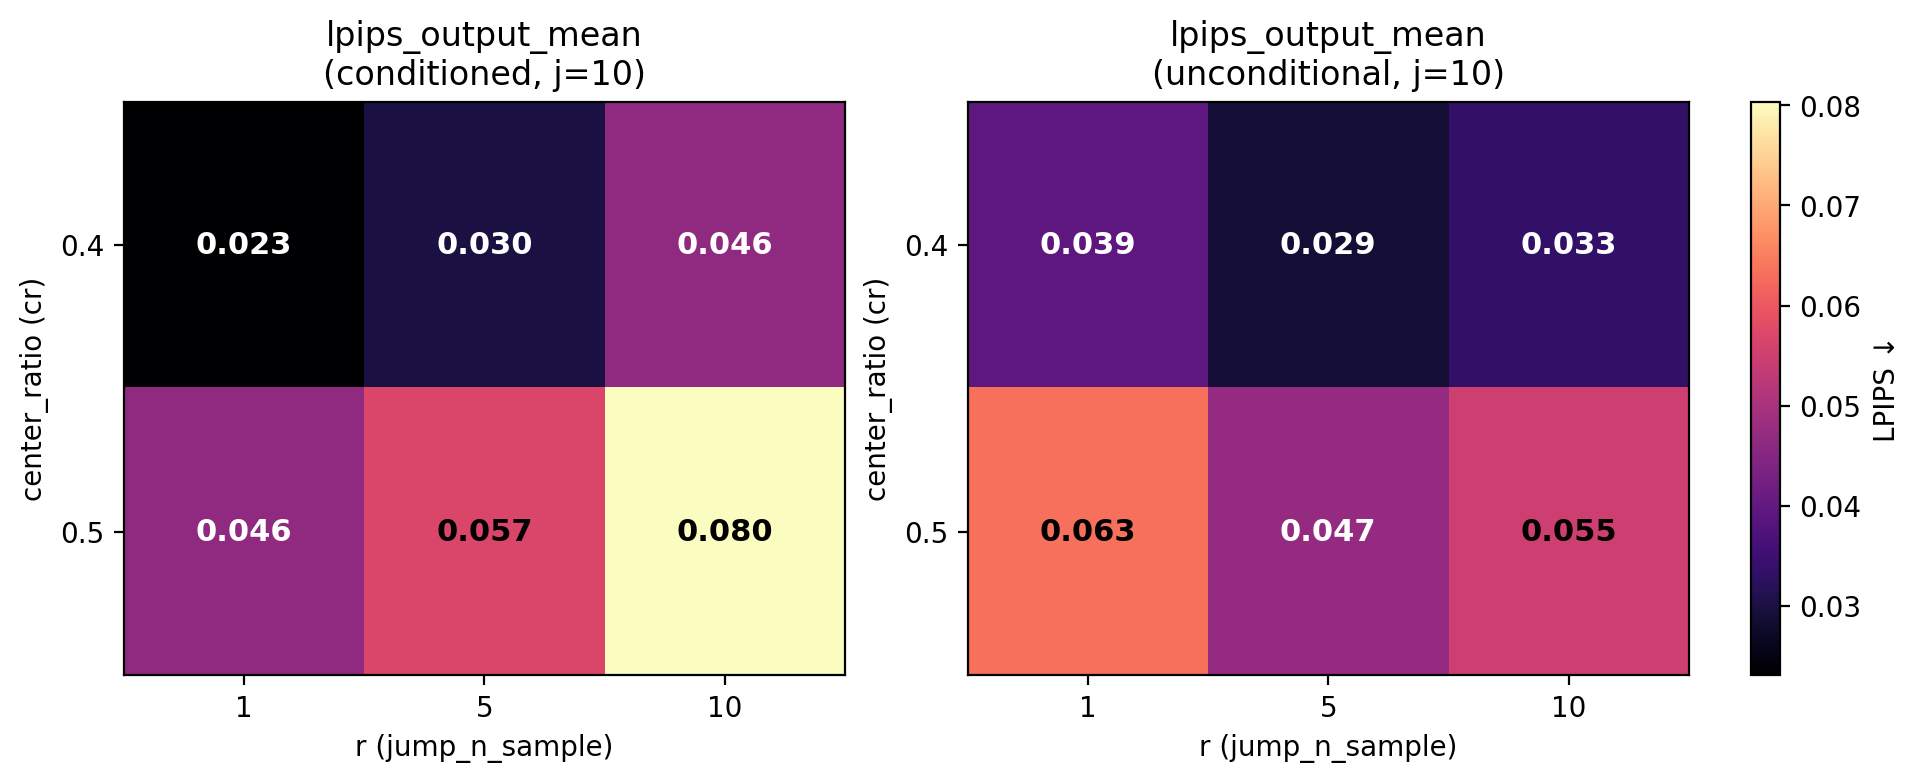
\includegraphics[width=0.98\linewidth]{figures/heatmap_lpips_output_mean_cr040_050_cond_vs_uncond_j10.png}
  \caption{Mean LPIPS (lower is better) over center-mask inpainting as a function of resampling count $r$ ($j{=}10$).
  Left: our conditioned DDPM. Right: our unconditional DDPM.
  Trends oppose: conditioned quality degrades with $r$; our unconditional quality improves from $r{=}1$ to $r{=}5$.}
  \label{fig:lpips-heatmap}
\end{figure}

\subsection{Qualitative evidence on our models}
\label{sec:qualitative}
Figures~\ref{fig:cond-r} and~\ref{fig:uncond-r} illustrate the same interaction on our own trained models.
Our conditioned outputs at $r{=}1$ are typically coherent; increasing to $r{=}10$ introduces washed-out / over-harmonized fills and visible degradation on several identities (Figure~\ref{fig:cond-r}).
Our unconditional model at $r{=}1$ often shows blotchy skin and hard seams; raising $r$ improves boundary harmony and facial structure (Figure~\ref{fig:uncond-r}).

\subsection{External qualitative check (RePaint CelebA-HQ)}
\label{sec:external}
Figure~\ref{fig:external-repaint} provides an independent check: RePaint's original pretrained (unconditional) CelebA-HQ checkpoint shows no comparable degradation under the same resampling sweep---in fact quality improves with $r$---suggesting the harm we observe on large centers is tied to \emph{mask conditioning} rather than to our specific architecture or training setup.
This figure is \textbf{not} our unconditional $64{\times}64$ model (Figure~\ref{fig:uncond-r}).
It uses RePaint's publicly released pretrained checkpoint at $256{\times}256$, with a respaced $T{=}100$ schedule, $j{=}10$, $r\in\{1,5,10\}$, and $n{=}8$ samples on a fixed identity with a lower-face (surgical-mask-style) hole.
The run is qualitative only (no PSNR/LPIPS) and should not be read as another cell of Table~\ref{tab:resampling-delta}.

% [H] preserves source order: external remnant above Figure 2, then brush + Table 2.
% Larger height fills the previous bottom gap on this page.
\begin{figure}[H]
  \centering
  \vspace{-0.5em}
  \begin{minipage}[t]{0.48\textwidth}
    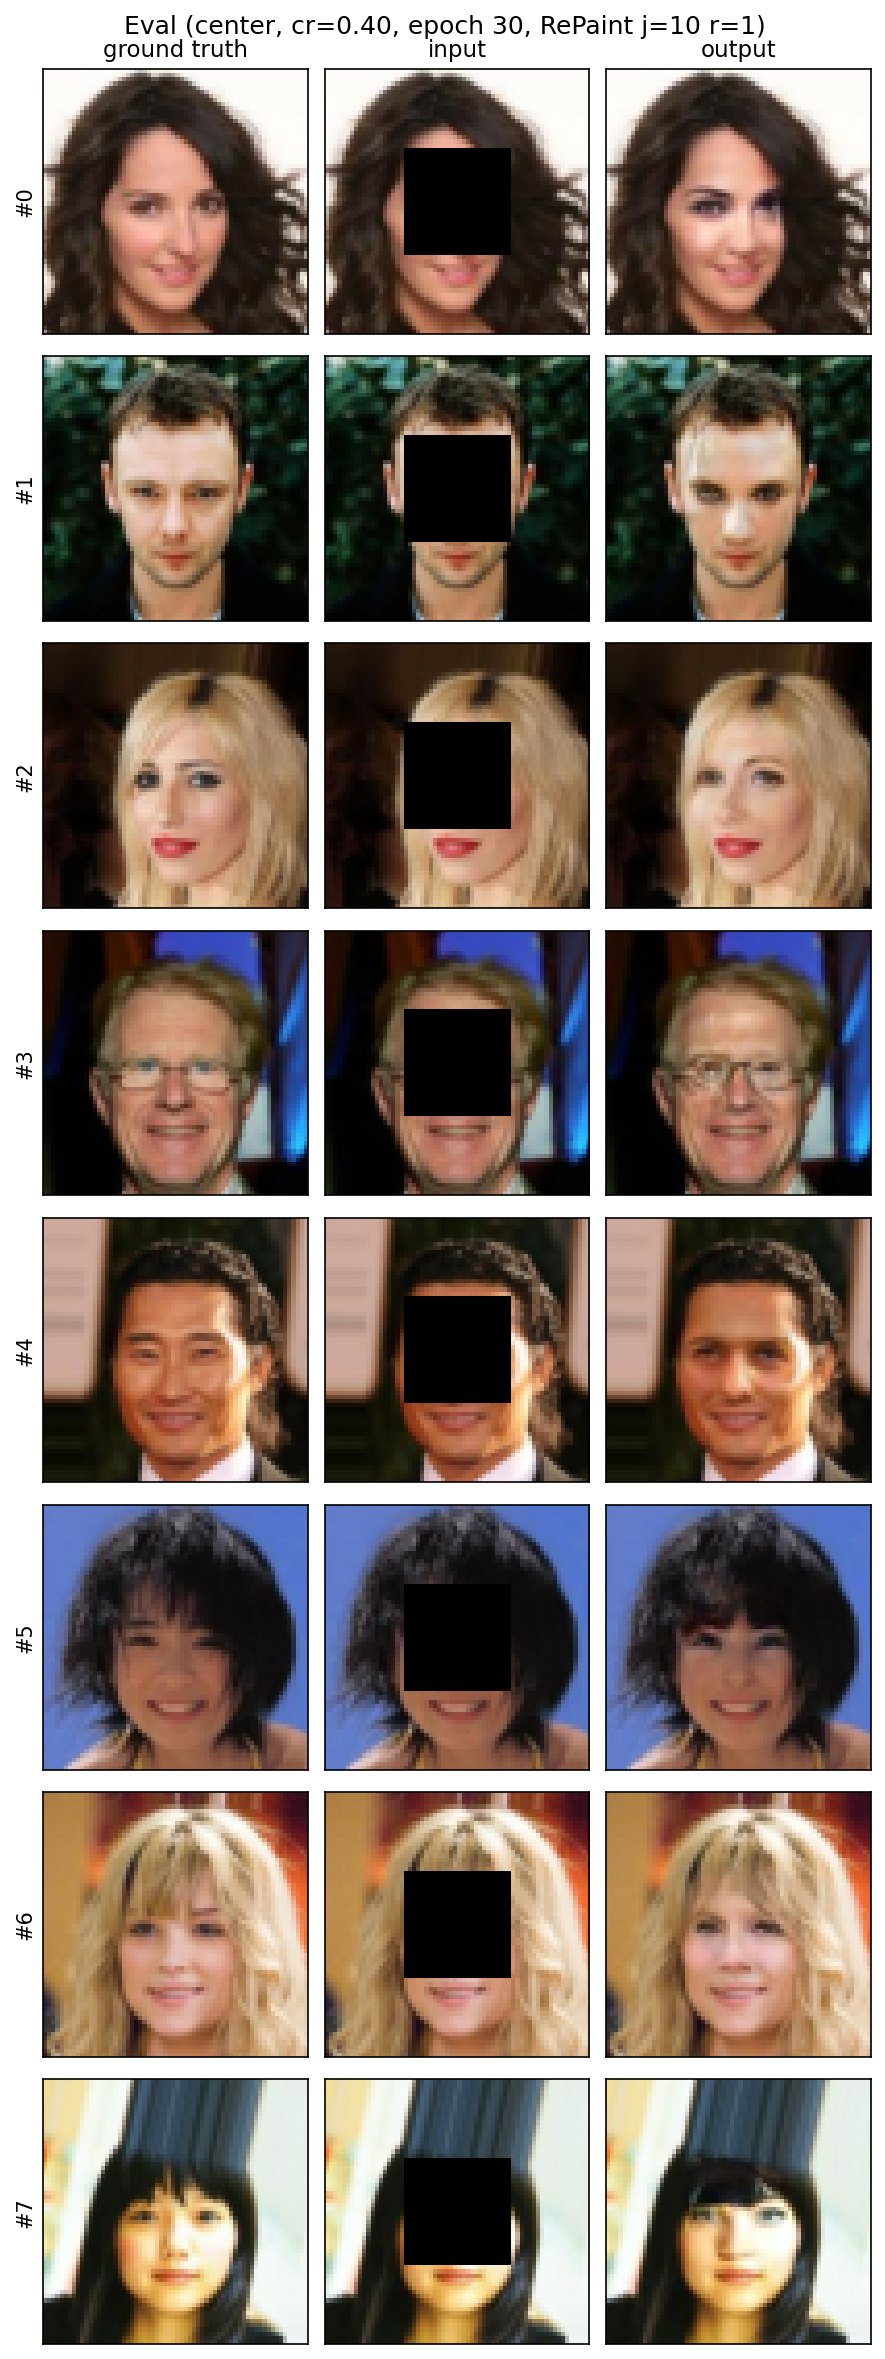
\includegraphics[width=\linewidth,height=0.41\textheight,keepaspectratio]{figures/eval_center_cr040_epoch_030_j10r1_grid.png}
    \vspace{-0.4em}
    \centerline{\small (a) Our conditioned, $r{=}1$}
  \end{minipage}
  \hfill
  \begin{minipage}[t]{0.48\textwidth}
    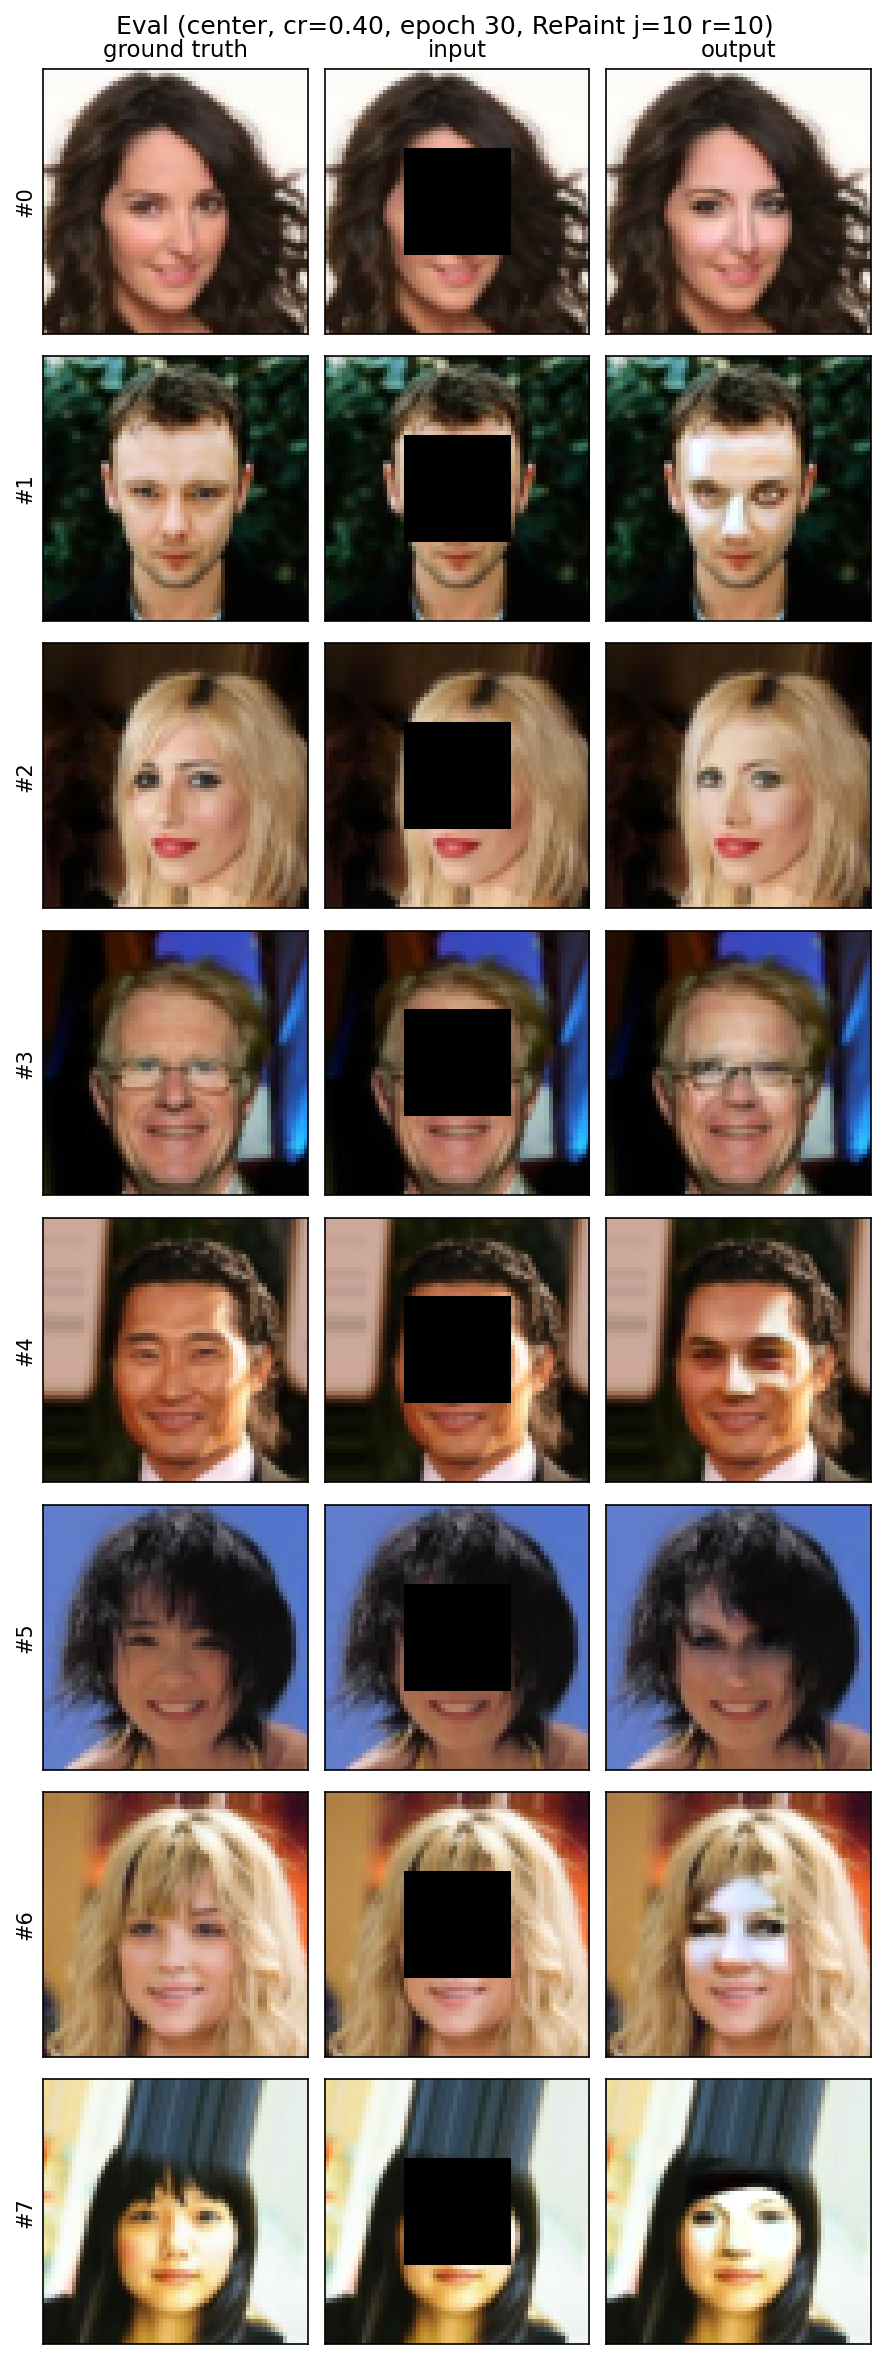
\includegraphics[width=\linewidth,height=0.41\textheight,keepaspectratio]{figures/eval_center_cr040_epoch_030_j10r10_grid.png}
    \vspace{-0.4em}
    \centerline{\small (b) Our conditioned, $r{=}10$}
  \end{minipage}
  \caption{Our conditioned CelebA model (epoch~$30$, $64{\times}64$), center $\mathrm{cr}{=}0.40$, $j{=}10$, full $T{=}1000$.
  Increasing $r$ from $1$ to $10$ tends to hurt fill quality.}
  \label{fig:cond-r}
\end{figure}

\subsection{Brush-mask control: the effect is contiguous-hole specific}
\label{sec:brush-null}
A natural confound is masked \emph{area}: perhaps any hole with $\mathrm{cr}{\approx}0.40$ coverage would show the same conditioned $r$-harm.
To test this, we evaluate the conditioned epoch-$30$ model on \textbf{brush} masks whose coverage is matched to a $\mathrm{cr}{=}0.40$ center hole, using the same paired protocol ($n{=}32$, $j{=}10$, $\Delta{=}\mathrm{metric}(r{=}10)-\mathrm{metric}(r{=}1)$, per-sample reseeding).
Table~\ref{tab:brush-null} reports a clean \textbf{null}.
Mean PSNR is essentially unchanged ($38.13\to38.43$\,dB):
$\Delta\mathrm{PSNR}{=}{+}0.30$\,dB with a 95\% CI that includes zero ($[{-}0.61,{+}1.20]$), $p{=}0.51$, and a negligible effect size (Cohen's $d{=}{+}0.12$).
$\Delta$LPIPS is likewise non-significant ($p{=}0.25$, $d{=}{+}0.21$).
Hole-PSNR differences match image-PSNR exactly under this protocol, as expected when only the masked region changes.
Increasing $r$ therefore neither reliably helps nor hurts under sparse, non-contiguous occlusion at matched coverage---while still costing ${\approx}10{\times}$ NFEs/$\,$wall-clock (Section~\ref{sec:cost}).
This rules out ``masked pixel count alone'' as the explanation for Table~\ref{tab:resampling-delta}:
the conditioned degradation under resampling is specific to \emph{large contiguous} holes, where RePaint's repeated re-harmonization has a coherent region to overwrite, not to brush strokes that leave dense local context.

\begin{table}[H]
  \centering
  \caption{Brush-mask control on the conditioned epoch-$30$ model ($n{=}32$, $j{=}10$).
  Coverage matched to center $\mathrm{cr}{=}0.40$.
  $\Delta{=}\mathrm{metric}(r{=}10)-\mathrm{metric}(r{=}1)$.
  Neither PSNR nor LPIPS changes significantly.}
  \label{tab:brush-null}
  \begin{tabular}{lcccc}
    \toprule
    Metric & $\Delta$ & 95\% CI & $p$ & Cohen's $d$ \\
    \midrule
    PSNR (dB) & $+0.30$ & $[-0.61,+1.20]$ & $0.51$ & $+0.12$ \\
    LPIPS & $+0.0006$ & $[-0.0005,+0.0017]$ & $0.25$ & $+0.21$ \\
    \bottomrule
  \end{tabular}
\end{table}

% No \clearpage here: prior \clearpage + oversized [H] produced a blank page.
\begin{figure}[H]
  \centering
  \begin{minipage}[t]{0.48\textwidth}
    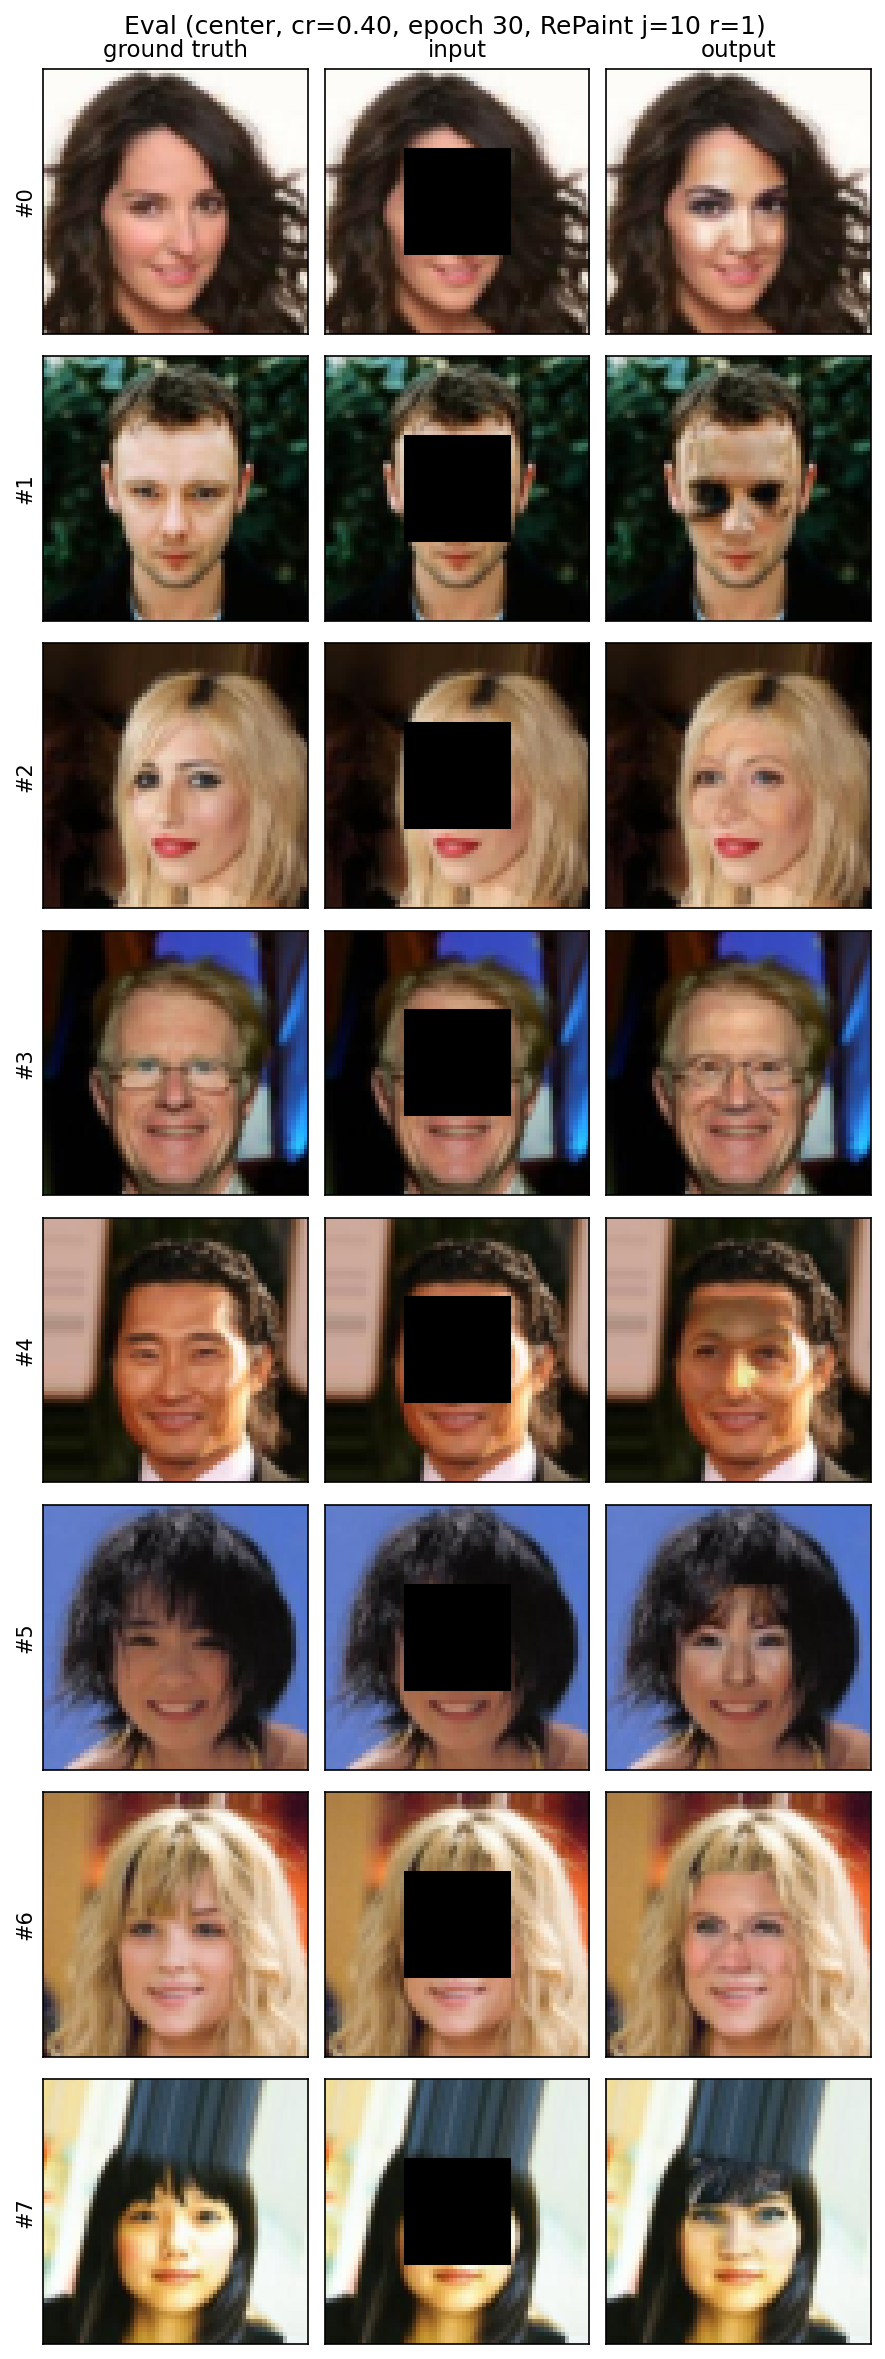
\includegraphics[width=\linewidth,height=0.40\textheight,keepaspectratio]{figures/eval_center_cr040_epoch_030_j10r1_uncond_grid.png}
    \vspace{-0.4em}
    \centerline{\small (a) Our unconditional, $r{=}1$}
  \end{minipage}
  \hfill
  \begin{minipage}[t]{0.48\textwidth}
    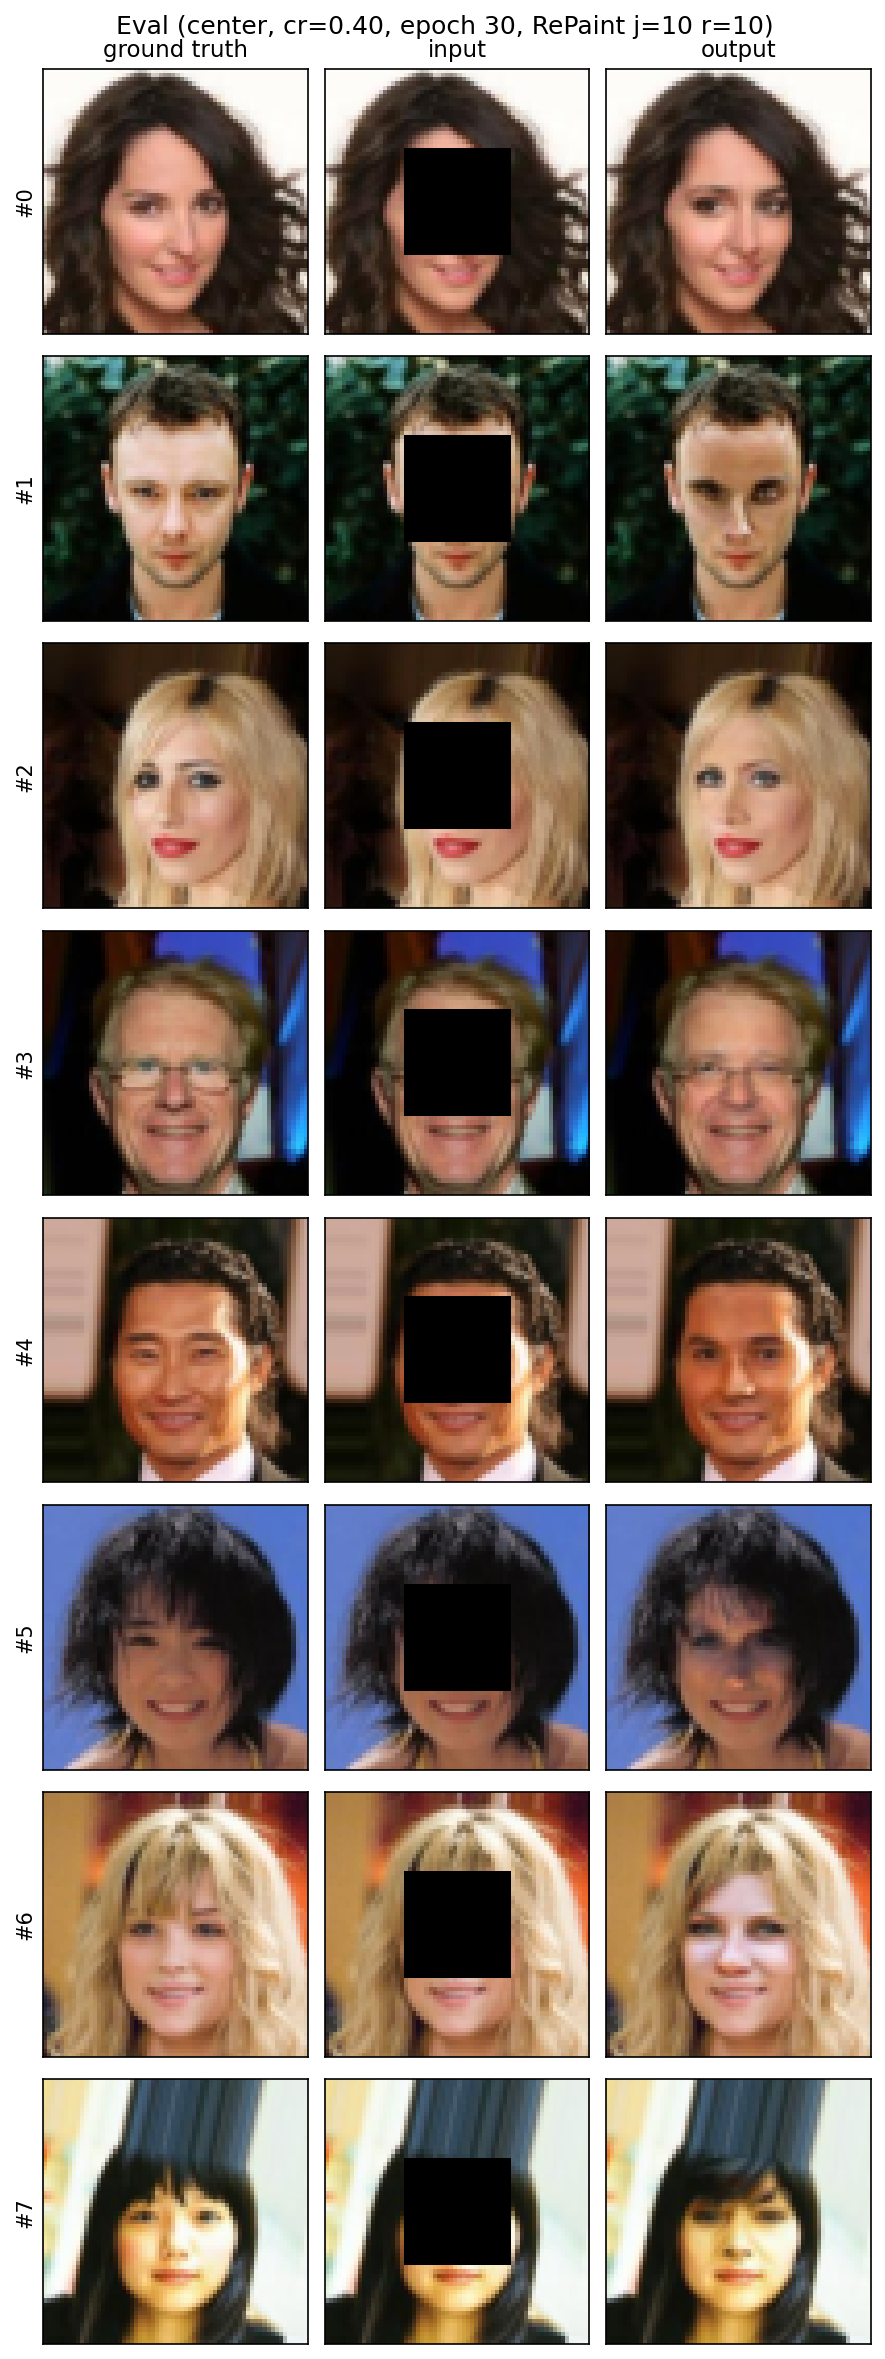
\includegraphics[width=\linewidth,height=0.40\textheight,keepaspectratio]{figures/eval_center_cr040_epoch_030_j10r10_uncond_grid.png}
    \vspace{-0.4em}
    \centerline{\small (b) Our unconditional, $r{=}10$}
  \end{minipage}
  \caption{Our unconditional CelebA model (epoch~$30$, $64{\times}64$), center $\mathrm{cr}{=}0.40$, $j{=}10$, full $T{=}1000$.
  Higher $r$ improves harmony relative to $r{=}1$ (Table~\ref{tab:resampling-delta} uses $r{=}5$ as the endpoint for our unconditional model).}
  \label{fig:uncond-r}

  \vspace{0.3em}

  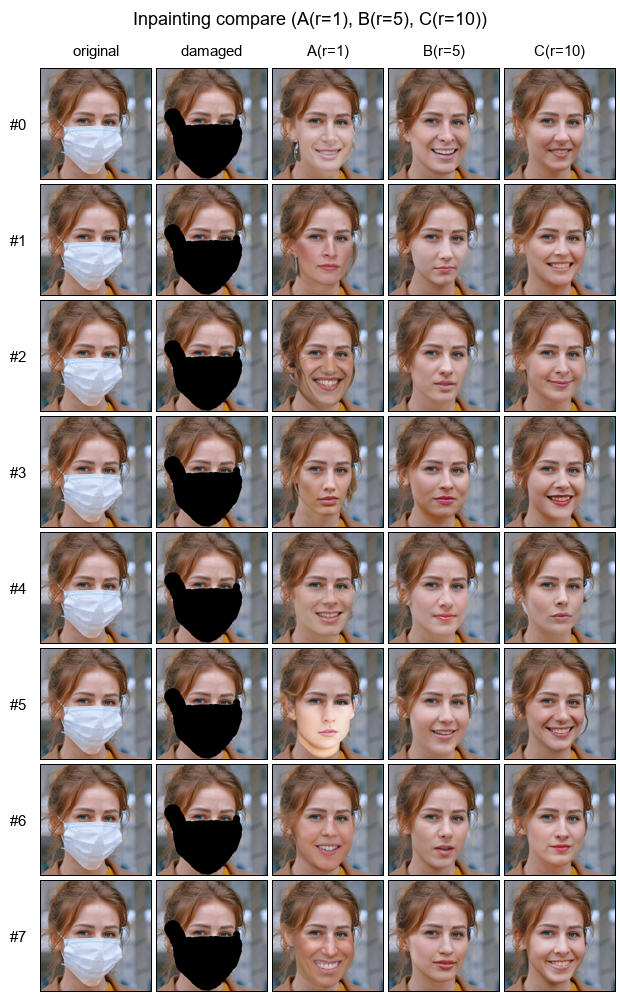
\includegraphics[width=0.98\textwidth,height=0.40\textheight,keepaspectratio]{figures/compare_ABC_grid.png}
  \caption{External qualitative check: RePaint's pretrained unconditional CelebA-HQ checkpoint ($256{\times}256$), \emph{not} our unconditional epoch-$30$ $64{\times}64$ model.
  Fixed identity, lower-face mask, respaced $T{=}100$, $j{=}10$, $n{=}8$.
  Columns: $r{=}1$, $r{=}5$, $r{=}10$.
  Higher $r$ improves seam consistency; unlike our conditioned model, there is no $r$-induced degradation.}
  \label{fig:external-repaint}
\end{figure}

\subsection{Compute cost of resampling}
\label{sec:cost}
Table~\ref{tab:nfe-cost} reports wall-clock and NFE cost as a function of $r$.

\begin{table}[H]
  \centering
  \caption{Inference cost vs.\ resampling count $r$ ($T{=}1000$, $j{=}10$). Ratios are relative to $r{=}1$.}
  \label{tab:nfe-cost}
  \begin{tabular}{rrrrr}
    \toprule
    $r$ & NFEs & NFE ratio & Wall-clock (s/img) & Time ratio \\
    \midrule
    $1$  & $1{,}000$ & $1.0{\times}$ & $14.1$ & $1.0{\times}$ \\
    $5$  & $4{,}960$ & $5.0{\times}$ & $70.8$ & $5.0{\times}$ \\
    $10$ & $9{,}910$ & $9.9{\times}$ & $149.7$ & $10.6{\times}$ \\
    \bottomrule
  \end{tabular}
\end{table}

Cost scales nearly linearly: $r{=}10$ requires ${\approx}9.9{\times}$ U-Net calls and ${\approx}10.6{\times}$ wall-clock time relative to $r{=}1$.
Combined with Table~\ref{tab:resampling-delta}, this yields a sharp practical conclusion for conditioned models: increasing $r$ can simultaneously \emph{worsen} quality and multiply inference cost by an order of magnitude.
For our unconditional model, moderate resampling ($r{=}5$) remains the operating point that improves quality, at about $5{\times}$ the cost of $r{=}1$.

\subsection{Takeaway}
\label{sec:takeaway}
RePaint resampling is not a universally beneficial hyperparameter.
Under matched seeds and identical images, its sign flips with the training regime: it helps the unconditional prior (as in the original RePaint setting) but hurts a mask-conditioned DDPM that already observes $(\tilde{x}_0,m)$ during reverse sampling.
The brush-mask null (Section~\ref{sec:brush-null}) further shows that the conditioned harm is tied to contiguous hole geometry, not coverage alone.
Reporting a single default $(j,r)$ across both regimes therefore conflates two different operating regimes---and, for conditioned models on large centers, can purchase worse images at substantially higher compute.

\section{Discussion}
\label{sec:discussion}

\subsection{What needs explaining}
The empirical pattern is sharp.
On large contiguous center holes, increasing RePaint's resampling count $r$ \emph{hurts} our mask-conditioned DDPM and \emph{helps} our unconditional DDPM (Table~\ref{tab:resampling-delta}, Figures~\ref{fig:cond-r} and~\ref{fig:uncond-r}).
Matched-coverage brush masks show no significant $r$ effect (Table~\ref{tab:brush-null}).
RePaint's own pretrained unconditional CelebA-HQ checkpoint likewise improves with $r$ (Figure~\ref{fig:external-repaint}).
We interpret this as a mismatch between RePaint's inference-time correction loop and how much measurement information the network already receives during each denoising step.

\subsection{Unconditional: resampling as alternating projections}
\label{sec:alt-proj}
In the classic RePaint setting the U-Net never sees a mask: $\varepsilon_\theta=\varepsilon_\theta(x_t,t)$.
Its reverse step proposes a full-image update $\hat{x}_{t-1}^{\mathrm{unk}}$; consistency with known pixels is enforced only by the stitch~\eqref{eq:stitch}, and when $r{>}1$ by forward jumps~\eqref{eq:jump}.
Writing $P_{\mathrm{prior}}(x_t)$ for one reverse (denoising) step that uses $\varepsilon_\theta(x_t,t)$, and $P_{\mathrm{data}}$ for the known-pixel stitch, a resampling cycle is the composition
\begin{align}
  x_{t-1}
  &\leftarrow
  \underbrace{m\odot q(x_0,t{-}1)+(1-m)\odot P_{\mathrm{prior}}(x_t)}_{\text{known-pixel projection }P_{\mathrm{data}}},
  \label{eq:proj-data}\\
  x_{t}
  &\leftarrow
  \underbrace{\sqrt{1-\beta_{t}}\,x_{t-1}+\sqrt{\beta_{t}}\,\varepsilon}_{\text{re-noise / jump}},
  \qquad \varepsilon\sim\mathcal{N}(0,I),
  \label{eq:proj-jump}
\end{align}
repeated within the RePaint $(j,r)$ schedule.
This is an instance of \emph{alternating projections}: $P_{\mathrm{prior}}$ moves toward the learned image manifold, $P_{\mathrm{data}}$ projects back onto the known-pixel constraint, and~\eqref{eq:proj-jump} reopens the hole so the pair can be applied again.
Without those projections, the hole and the context disagree at the boundary---hence the blotchy seams at $r{=}1$ and the clear gain from $r{=}5$ on our unconditional model (and on the external CelebA-HQ checkpoint).
Resampling is doing real work that the architecture does not otherwise provide.

\subsection{Conditioned: a static conditioning channel already carries the constraint}
Our conditioned model instead predicts $\varepsilon_\theta(x_t,t,\tilde{x}_0,m)$ from the concatenation $(x_t,\tilde{x}_0,m)$ at every reverse step.
Known content is therefore not only an after-the-fact constraint $P_{\mathrm{data}}$; it is a \emph{static conditioning channel} the network was trained to read while predicting $\varepsilon$.
Under that training regime, a single application of~\eqref{eq:stitch} at $r{=}1$ is usually enough: the reverse process is already steered by $(\tilde{x}_0,m)$, and large-center fills at $r{=}1$ are coherent (Figure~\ref{fig:cond-r}a).

Raising $r$ re-imposes the alternating-projection loop~\eqref{eq:proj-data}--\eqref{eq:proj-jump} on top of that channel.
Each extra jump re-noises the hole, re-denoises, and re-applies $P_{\mathrm{data}}$---repeatedly overwriting a fill that the conditioned predictor had already committed to.
We hypothesize that this second consistency mechanism is largely redundant for a mask-conditioned $\varepsilon_\theta$, and on large contiguous holes it is actively harmful: the hole is big enough that re-harmonization can replace a sharp, identity-specific completion with an over-smoothed / washed-out compromise (Figure~\ref{fig:cond-r}b).
In short, alternating projections fix a missing constraint in the unconditional case; they fight a constraint that is already inside the network in the conditioned case.

\subsection{Why the brush null fits}
If the harm were merely ``more compute'' or ``any missing pixels,'' matched-coverage brush masks should degrade similarly under $r{=}10$.
They do not (Table~\ref{tab:brush-null}).
Brush strokes leave dense local context adjacent to every missing pixel, so both the static conditioning channels and a single stitch already determine the fill; there is little contiguous region for repeated re-harmonization to rewrite.
The conditioned $r$-harm is therefore geometry-specific: it tracks large contiguous holes where RePaint's loop has a coherent interior to overwrite, not masked area alone.

\subsection{Practical implication}
RePaint's default $(j,r)$ was designed for unconditional generators.
Copying that recipe onto a Palette-style conditioned DDPM is not a neutral choice: on hard center masks it can cost ${\approx}10{\times}$ NFEs while lowering PSNR by ${\sim}2.7$\,dB.
A regime-aware rule is simpler---use moderate resampling for our unconditional model (and classic unconditional RePaint); prefer $r{=}1$ (noise-matched stitch only) for mask-conditioned models on large contiguous holes (brush/sparse masks are insensitive to $r$ either way, so $r{=}1$ is a safe default there too)---and report $(j,r)$ jointly with the training mode.

\subsection{Limitations of the mechanism story}
This account is an interpretation of paired ablations, not a proof of the internal computation.
We do not intervene on intermediate latents, ablate the conditioning channels at inference, or derive a formal fixed-point for the RePaint operator under concat-conditioning.
Alternative explanations remain open, including capacity limits that make repeated resampling amplify a bad mode.

\paragraph{Schedule granularity.}
A particularly natural alternative---raised by RePaint's own discussion of per-step harmonization budget under finer schedules---is that resampling benefits are schedule-specific rather than conditioning-specific.
Our headline grid (Table~\ref{tab:resampling-delta}) runs both of our models at full $T{=}1000$; the external check (Figure~\ref{fig:external-repaint}) uses a coarse respaced $T{=}100$ schedule but only for RePaint's pretrained CelebA-HQ checkpoint.
We therefore evaluate the conditioned model only at full $T{=}1000$; whether the resampling-harm effect weakens or disappears at coarser, respaced schedules (as in RePaint's original $T{=}250$ setting) remains untested and is a natural target for follow-up work.
That said, granularity alone does not explain the \emph{within}-schedule sign flip: at matched $T{=}1000$, the same $(j,r)$ recipe helps our unconditional model and hurts our conditioned one, which still points to conditioning as a driver even if schedule interacts with effect size.

What the present data do pin down is that sign flip, its concentration on contiguous holes, and the fact that RePaint's pretrained CelebA-HQ checkpoint does not show conditioned-style degradation under higher $r$.

\subsection{Scope limitations}
Beyond the mechanism caveats above, the study itself is narrow.
All quantitative claims use a single checkpoint epoch ($30$), one U-Net capacity recipe, and $64{\times}64$ CelebA only.
Paired tests use $n{=}32$ seed-matched images; effect sizes are large for the conditioned harm, but broader populations and datasets are untested.
Mask coverage is limited to center squares plus one brush control---not free-form or semantic masks at scale---and we do not ablate learned variance, classifier-free guidance, or latent-space / Stable-Diffusion-style inpainting pipelines.
Wall-clock numbers are hardware-specific; NFE ratios are the portable cost measure.
These bounds do not overturn the paired interaction we report, but they limit how far the practical ``$r{=}1$ for conditioned models, moderate $r$ for our unconditional model'' rule should be extrapolated without further evidence.

\section{Conclusion}
\label{sec:conclusion}

We show that RePaint's resampling hyperparameter $r$ is not a universally beneficial default: under paired, seed-matched evaluation, increasing $r$ improves our unconditional DDPM but degrades a mask-conditioned DDPM on large contiguous holes, with effect sizes that are both large and highly significant.
A matched-coverage brush-mask control and an external check on RePaint's own pretrained CelebA-HQ checkpoint rule out masked area and architecture-specific artifacts as explanations, pointing instead to mask conditioning itself as the driver.
Because the best-performing setting for conditioned models ($r{=}1$) is also the cheapest, the practical rule is simple: match $(j,r)$ to the training regime rather than copying a single default across both.
Whether this interaction persists at coarser respaced schedules, larger architectures, or other datasets remains open, and we see the conditioning$\times$resampling interaction identified here as a concrete, testable starting point for that follow-up work.


{\small
\bibliographystyle{plainnat}
\bibliography{refs}
}

\end{document}
